\documentclass[]{final_report}
\usepackage{graphicx}
\usepackage{hyperref}
\usepackage[final]{pdfpages}
\usepackage{natbib}
\usepackage{booktabs}
\usepackage{multirow}
\usepackage{framed}
\usepackage{caption}
\usepackage{tikz}
\usetikzlibrary{timeline}


%%%%%%%%%%%%%%%%%%%%%%
%%% Input project details
\def\studentname{James King}
\def\reportyear{2018}
\def\projecttitle{Cooperative Strategies in Multi-Agent Systems}
\def\supervisorname{Kostas Stathis}
\def\degree{BSc (Hons) in Computer Science}
\def\fullOrHalfUnit{Full Unit} % indicate if you are doing the project as a Full Unit or Half Unit
\def\finalOrInterim{Interim Report} % indicate if this document is your Final Report or Interim Report

\begin{document}

\maketitle

%%%%%%%%%%%%%%%%%%%%%%
%%% Declaration

\chapter*{Declaration}

This report has been prepared on the basis of my own work. Where other published and unpublished source materials have been used, these have been acknowledged.

\vskip3em

Word Count: 

\vskip3em

Student Name: \studentname

\vskip3em

Date of Submission: 

\vskip3em

Signature:

\newpage

%%%%%%%%%%%%%%%%%%%%%%
%%% Table of Contents
\tableofcontents\pdfbookmark[0]{Table of Contents}{toc}\newpage

%%%%%%%%%%%%%%%%%%%%%%
%%% Your Abstract here

\begin{abstract}

\end{abstract}
\newpage

\chapter{Aims, Objectives and Literary Survey}
\section{The Problem}
\label{section:problem}
To understand the aims and objectives of this project we must first grasp the history of the study of interaction between biological and computational agents (often known as intelligent agents in the field of computer science). It is important to distinguish between biological and computational agents as the study of natural selection and the evolution of cooperation in biological agents has a long and separate history from the study of intelligent agents in computer science.\\
The background I am about to explain is covered in my first two reports (included in the appendix in chapter~\ref{appendix}): `report on the evolution of cooperation in relation to game-theory and different game-theoretic mechanisms to aid it' and `report on indirect reciprocity, strategies for agents and the development of a concrete model to implement'. I will be applying this knowledge in a more convenient format for the interim report here, but if you are interested in reading a more in-depth study by myself on this topic, I suggest reading these two.\\
As explained in my first report (on the evolution of cooperation in relation to game-theory and different game-theoretic mechanisms to aid it) early Darwinian evolutionary theory was groundbreaking, but both opponents and even proponents of evolution such as Peter Kropotkin~\cite{kropotkin1902mutual} (a Russian evolutionary scientist and political activist) found it fell short in explaining cooperative phenomena.\\
Cooperation is the idea of helping others at a detriment or cost to yourself. Of course, this is a key part of the natural world, like the act of parents supporting their children and vice-versa in human family groups. There are even interspecies examples such as that of the Meerkat and Drongo Bird~\cite{bbcafrica}.\\
The problematic question posed by this phenomena is that natural selections idea: the survival of the fittest~\cite{spencer1864principles}, pushes individuals to compete for resources, so why does cooperation exist when there is a process actively pushing for competition? How did cooperation evolve in a world focused on competition?

\section{Cooperation Aids}
There have been a number of attempts to explain the phenomena of cooperation~\cite{kropotkin1902mutual, selfish_gene, evolution_of_cooperation, five_rules_coop}. Richard Dawkins in his book the selfish gene~\cite{selfish_gene} attempted to explain the idea that the real replicator in natural selection is the gene which is self-interested in replication. As such, individuals are driven to working towards replication of the gene, not to improving our own personal fitness\\
This idea comes under the banner of Kinship Theory, highlighted by Axelrod and Hamilton in their paper the evolution of cooperation~\cite{evolution_of_cooperation} as one of the theories seeking to explain cooperation. Hamilton wrote a paper on Kinship Theory earlier in his academic career~\cite{kinhamilton} explaining his version of Kinship Theory in which agents are encouraged to cooperate as they are interested in improving `inclusive fitness' over their own individual fitness. Inclusive fitness refers to the fitness of both them and their relatives, the closer the relative the more they have an effect on an agent's inclusive fitness.\\
The main mechanism highlighted by Axelrod and Hamilton~\cite{evolution_of_cooperation} is, in popular culture, known as the iterated prisoner's dilemma. The iterated prisoner's dilemma uses the idea of direct reciprocity to aid in the evolution of cooperation. This idea being: if I scratch your back you'll scratch  mine. In a round of the prisoner's dilemma, both agents simultaneously choose whether to cooperate or defect. A single prisoner's dilemma round provides no aid, but if the rounds are repeated agents are encouraged to cooperate if historically there has been cooperation from the other agents they are interacting with. Another reason to cooperate is the payoff matrix given in table~\ref{tab:ipdpayoffmatrix}. As you can see multiple rounds of both agents cooperating gives both higher social welfare (overall points accrued~\cite{kostas_deductive}) and greater individual payoff than multiple rounds of mutual defection.
\begin{framed}
	\begin{center}
		\begin{tabular}{c|c|c}
		\multirow{2}{*}{Player A} & \multicolumn{2}{c}{Player B}\\		
		& Cooperation & Defection\\
		\hline
		\multirow{2}{*}{Cooperation} & A=3 & A=0\\
		& B=3 & B=5\\
		\hline
		\multirow{2}{*}{Defection} & A=5 & A=1\\
		& B=0 & A=1\\
		\end{tabular}
		\captionof{table}{The payoff matrix in a typical iterated prisoner's dilemma game (such as Axelrod and Hamilton's). A=x, B=y where x denotes the payoff for A and y the payoff for B.}
		\label{tab:ipdpayoffmatrix}
	\end{center}	
\end{framed}
Direct reciprocity and Kinship Theory (or kin selection) are 2 of the five rules presented in Martin A. Nowak's paper `Five Rules for the evolution of cooperation'~\cite{five_rules_coop}. The other 3 also use different versions of reciprocity mechanisms. Network reciprocity is similar to the iterated prisoner's dilemma. Axelrod and Hamilton's approach~\cite{evolution_of_cooperation} uses a round-robin tournament where all players interact with every other player. Network reciprocity is set aside from this as it is played on a graph with players as the nodes, and the edges denoting who interacts with whom.\\
Another of the five rules, group selection, builds upon indirect reciprocity. This mechanism separates a population out into smaller subpopulations. The players in these subpopulations only interact and reproduce within their subpopulation group. These group sizes fluctuate based on how fast agents reproduce inside them (dependent on the agents' fitness scores). If a group gets to a certain size it has a chance of splitting and when one group splits another group is removed. The effect being selection on two levels: individually and between groups, aiding the evolution of cooperation.\\
The last mechanism presented by Nowak and one I am most interested in is indirect reciprocity. The idea behind this mechanism is slightly less intuitive than direct reciprocity: If I scratch your back hopefully later on someone else will remember that and scratch my back. Actions in indirect reciprocity are different to direct reciprocity as they do not involve both agents acting. Only the donor of the donor-recipient interaction pair can choose to cooperate or defect, the payoffs of which are presented in table~\ref{tab:indirectpayoffmatrix}.
\begin{framed}
	\begin{center}
		\begin{tabular}{c|c|c}
		\multirow{2}{*}{Donor Action} & \multicolumn{2}{c}{Payoffs}\\		
		& Donor & Recipient\\
		\hline
		Cooperation & -1 & 2\\
		\hline
		Defection & 0 & 0\\
		\end{tabular}
		\captionof{table}{The common payoff for most indirect reciprocity models}
		\label{tab:indirectpayoffmatrix}
	\end{center}	
\end{framed}
The indirect reciprocity mechanism utilizes the idea of reputation, cooperative acts may result in bettering the donor's reputation whereas defecting may result in a loss of reputation. How agents view the reputation of another depends upon their implementation, two important implementations described in my second report are the standing strategy~\cite{leimarhammer} and using image scores~\cite{evol_indirect_image}. Agents have the opportunity to base their decisions on these reputations. It was also put forward by Sommerfeld \textit{et al.}~\cite{gossip_alt} that the social action of gossip can help agents spread information in regards to agents reputations.

\section{Theory Surrounding Intelligent Agents and Multi-Agent Systems}
The theory I will cover here is mostly covered in my third report (also in the appendix chapter~\ref{appendix}) but here I have applied the information in a relevant way to introduce my project. Agents, as described by Russell and Norvig, are anything that perceives and acts upon its environment~\cite{russell2016artificial}. Agents can be built using a number of architectures, some of which are seemingly more intelligent than others. Russell and Norvig highlight 5 such architectures ranging from agents which simply act in reflex to their environment to agents that actively learn from their percepts.\\
This could be considered a `weak' notion of agency even in comparison to Wooldridge and Jennings' `weak' notion of agency defined in their paper: ``Intelligent agents: theory and practice''~\cite{wooldridge_jennings_1995}. This paper stipulates agents must be able to exhibit these 4 properties: autonomy, social ability, reactivity and proactivity.\\
Autonomy is considered to be operating without direct human or other agent intervention, with the agent having control over their internal state and actions. Social ability is defined as the ability of agents to interact with other agents (possibly biological) using an agent communication language. Reactivity is the ability to perceive their environment and act upon the changes in it. Proactivity makes Wooldridge and Jennings' notion stronger than Russell and Norvig's as it stipulates agents must not simply be reactive to their environment but are also able to exhibit goal-directed behaviour.\\
To be able to satisfy the properties laid out by Wooldridge and Jennings and the definition of an agent from Russell and Norvig agents need an environment to reside in. The possible environments are endless. An agent is built to work in a specific environment, the reason for an agents existence varies but often agents will attempt to complete specific tasks delegated to them.\\
Multi-agent systems are systems consisting of a combination of an environment and a number of agents perceiving and acting within it. Interactions can generally occur between both the environment and other agents in the system.


\section{Relevance of The Problem and Indirect Reciprocity to Multi-Agent Systems}
The societies which are simulated in the theories and experiments presented by Axelrod, Hamilton and Nowak~\cite{evolution_of_cooperation, five_rules_coop} are strikingly similar to multi-agent systems. The similarity is that they are groups of players residing in an environment interacting with each other. This leads naturally to using these game-theoretic approaches to modelling interactions in multi-agent systems.\\
As agents act autonomously in a multi-agent system, why should one agent cooperate with another at a cost to themselves? Of course from our viewpoint, we can see the possibilities that if agents work together they can accomplish so many brilliant things. From the agent's viewpoint though, why should that agent trust that if they cooperate, their good actions will not be taken advantage of?\\
This is the problem in section~\ref{section:problem} reformulated for multi-agent systems. From a developer's perspective who is working on these sorts of systems, their goal is to encourage cooperation between agents but also not leave their agents or system of agents open to abuse. How can developers achieve this goal?\\
One way to approach this problem is to study how other environments have achieved this. One such environment that has achieved the evolution of cooperation, that we have identified earlier in this report, is the environment we live in, nature itself. Though nature encourages competition it has also led to cooperation between biological agents. So how can we learn from the processes nature employs?\\
We can apply the processes identified by game-theory and Kinship Theory to model multi-agent systems by implementing multi-agent systems that run these processes. Using a similar mechanism to indirect reciprocity Mui \textit{et al.}~\cite{Mui:2002:NRM:544741.544807} explored reputations role in the evolution of cooperation in multi-agent systems. The paper uses a number of different notions for reputation, one similar to Nowak's observer-based reputation, where an agent changes their view of another agent depending on the actions it views of the other agent. Their experiments found a large number of interactions were needed per generation for cooperative agents to dominate.\\
The mechanism/process I have chosen and outlined in my report on indirect reciprocity was chosen as I believe it applies well to multi-agent systems for a number of reasons. Firstly agents who interact across large networks such as the internet may never interact again, so it is imperative to have a strategy for deciding on how to act in these singular interactions. My models use of indirect reciprocity and reputation will allow us to study specifically these sort of `sparse' interactions and the effectiveness of strategies in these interactions.\\
Another reason I believe my model matches multi-agent systems well is the social ability that it comes with. Nowak and Sigmund highlighted the importance of knowing another agents reputation to the success of the evolution of cooperation in an indirect reciprocity system~\cite{evol_indirect_image}. They found that the probability of knowing another agents reputation had to be greater than the cost to benefit ratio of the action for cooperation to evolve.\\
In my system agents who know each other will be able share information via gossip on other agents, this information increases the chances of knowing a certain agents reputation and in turn, helps defend against the generally cooperative or `nice' agents from being exploited. However, it also leads to another avenue of attack through spreading misinformation. This mechanism of information sharing could be used as a defence against exploitation, but it is important to understand how best to implement it and how effective it is before such an option is chosen.\\
One of the four properties laid out by Wooldridge and Jennings~\cite{wooldridge_jennings_1995} is autonomy, which includes control over the agent's own internal state. The fact that in my model reputation is not a centrally managed concept but is part of the internal state, brings the system closer to a truly decentralised multi-agent system architecture.\\
Though reproduction itself doesn't, in fact, occur in multi-agent systems it is likely that agent systems will be replaced and upgraded. The replacing systems will probably follow strategies that are known as effective by the developers. So my reproduction mechanism aims to show how this replacement will take place, by assigning more likelihood for reproduction of an agent to occur if the strategy is successful. The reproduction may tend towards a defecting agent if they are more successful and vice-versa.\\
For further information on my model please refer to my second report on indirect reciprocity, strategies for agents and the development of a concrete model to implement in the appendix in chapter~\ref{appendix}.

\section{Project Specification, Aims and Objectives}
As you can see the study of indirect reciprocity and other mechanisms is important for the development of multi-agent systems and the prevention of exploitation by malicious agents. My project is to work on studying the model of indirect reciprocity I have defined and it's effectiveness in aiding the evolution of cooperation.\\
I will be doing this by implementing the model as a multi-agent system with a variety of strategies including the image scoring discriminator and standing strategy described in my second report. The specification for my system design has been described in my third report. Further to the multi-agent system, I will be implementing a web application to run the environment, this web application will allow a user to select agents for their simulation and then run the simulation. The web application aims to act as an educational system on direct and indirect reciprocity (direct reciprocity has already been implemented using a preexisting library as a proof of concept for the web application).\\
After the simulation has ended a user will be redirected to an analysis of the simulation, where they will be able to examine the success of the model and strategies in regards to the evolution of cooperation. Analysis data will be held in a database for reuse later on. I will be using this system myself to examine the model and strategies effectiveness, alongside how the setting of parameters such as the number of interactions per generation are required for cooperation to evolve - as was examined by Mui \textit{et al.}~\cite{Mui:2002:NRM:544741.544807}.\\\\
To sum up my aims:
\begin{itemize}
	\item Implement the mechanism I have outlined in a multi-agent system
	\item Implement a number of strategies for use in the model
	\item Examine the relevance and success of the mechanism I have outlined in regards to the evolution of cooperation in multi-agent systems
	\item Examine the success of different strategies and trust models for agents in the system
	\item Explore how social ability/gossip can affect the evolution of cooperation in a multi-agent system
	\item Explore the various parameters that are important in the system in regards to what setting is required for cooperation to evolve
\end{itemize}

\chapter{Planning and Timescale}
Provide timeline of completed work and an updated one for next term.\\
Finished Project Plan October 4th.\\
Finished Nature Engine Proof of concept 22nd of October.\\
Finished prolog service on the 28th of October.\\
Defined model on November the 1st.\\
Environment design and partial implementation\\
\begin{framed}

\end{framed}



\chapter{Summary of Completed Work}
Relevance to project aims
\begin{itemize}
	\item Evolution of cooperation report
	\item Indirect reciprocity report
	\item System design report
	\item A prolog web app for proof of concept
	\item A flask web application to begin educational tool and as a proof of concept
	\item API documentation
	\item Agents service:
	\begin{itemize}
		\item Vertical slice of 3 strategies: perceive, revise, decide
		\item Use of mvfcec for revise
		\item Agent management
		\item Test agents revision
		\item Get strategies implementation
		\item 
	\end{itemize}
\end{itemize}
Agents service, flask web app, environment, two reports

\section{Proof of Concept}
\subsection{Proof Of Concepts}
After finishing my project plan I embarked on the implementation of two proof of concept programs. Both involved learning technologies that are new to me. The first proof of concept I had already begun work on in the summer was implementing a web application to select agents and parameters to run matches and tournaments of direct reciprocity using the Axelrod-Python library to run the matches and tournaments.\\
For this I used Python and learnt the Flask microframework to develop the web application alongside the SQLAlchemy ORM and SQLite for development. To learn the Flask microframework and it's ecosystem I took the course `The New and Improved Flask Mega Tutorial'~\cite{flask_tut}. This greatly improved my web development knowledge and skills, but I found I needed some more knowledge for developing front end to select a dynamic number of agents so took a crash course in React.js~\cite{react_crash_course}.\\
Using the skills I accrued from these two courses and my knowledge of direct reciprocity the Axelrod-Python library and Python itself I successfully developed the web application. This application uses a wide array of technologies such as Redis, Bootstrap and others previously mentioned. I feel that it really helped develop my skills in web development, which will be beneficial to using a nice graphical user interface for running and analysis of tournaments and also the educational aspects of my final product. \\
To run the web application which I have dubbed `The Nature Engine' if there is no database present (which would be the file app.db in the NatureEngineWebApp directory) activate the python virtual environment for the NatureEngine project and run the commands: flask db init, flask db migrate, flask db upgrade. To be able to run a direct reciprocity tournament there needs to be a redis worker active, to activate this firs activate the virtual environment and then run the command: rq worker nature\_engine\_tasks. You may notice that there is match analysis but no tournament analysis, this is coming soon as I decided to move on from the proof of concept to get the ball rolling in other activities.\\
My second proof of concept application was a small web service written in Prolog. Again the technologies used for this were new to me so I followed a tutorial `Creating Web Applications in SWI-Prolog'~\cite{swi_web_tut} and continuously consulted the SWI-Prolog documentation. The purpose of this proof of concept application was to practice and demonstrate that I can create web services using Prolog before I went ahead and developed the agents service.\\
This second proof of concept was successful and I proved to myself that I could create an adequate web service. The outcomes of this were a knowledge that I immediately put to use in creating the agents service and also a guide on how I can do this using the JSON format and certain methods of error handling etc.

\section{Practical}
Moving on from the proof of concept programs I started on design and implementation of the multi-agent system including the agents service and environment.
\subsection{Agents Service and API}
For SWI-Prolog there is a lack of an integrate project support environment or even an integrated development environment (except for in GNU EMACS which I do not have experience with). The tooling I have been using for the development of the agents service is the syntax highlighter in sublime text, and for testing the experiment bed (provided as part of the multi-valued fluent cached event calculus) and the Prolog unit-test framework. I have used this to test belief revision in the file tests.pl under the directory AgentsService/src/mvfcec/src. To run this compile the tests.pl in SWI-Prolog (tested on v7.6.4) and run the predicate run\_tests(percepts).\\
Further unit testing and dcumentation of the system is required to improve coverage and understandability of the code. However testing of the functionality of the system using API testing has been extensive, the API testing code can be found in the directory NatureEngineWebApp/tests/agents\_service\_testing. I decided to write my own testing using the python requests library and unittest framework instead of a tool such as Postman as I can easily commit the tests using git without needing to pay and the python requests library and unittest framework are both extremely easy and nice to use. I have also used these previously so they required no extra learning.\\
I have also create documentation for the API using the RESTful API Markup Language RAML (based on YAML). RAML has tooling surrounding it to easily convert a .raml file into a user understandable format, such as the raml2html tool that I have used to generate the file main.html under the directory AgentsService/api\_docs.\\
The API is designed to use the correct HTTP methods, use uniform resource indicators to access and manipulate resources and generally conform to RESTful API principles outlined at \url{https://restfulapi.net/}.\\
The agents service code for the web service side of the program has been based on my learning from the proof of concept prolog service. The code that runs the multi-valued fluent cached event calculus (mvfcec) has come from my supervisor Kostas Stathis. I have built on top of mvfcec with initiates\_at/3 predicates to define how an agent revises it's revises it's beliefs using mvfcec (this is in the AgentsService/src/revise.pl file). Revision of beliefs has been implemented for when an agent is in an interaction, and when a standing strategy agent (both trusting and distrusting variants) receives gossip and interaction observation percepts.\\
A whole vertical slice has been implemented for defector, cooperator and standing strategy strategies. This means that they can receive percepts (refer to AgentsService/src/percepts.pl file), revise their beliefs and decide on actions at specific timepoints based on their knowledge at that point (refer to AgentsService/src/actions.pl).\\
The agents are built in the deductive reasoning style and using the concepts of beliefs, commitments, capabilities and logical theories as described in my system design report.\\
Further to this vertical slice it is also possible to query agents beliefs on when they were a donor, recipient, when two believe they were both in an interaction together and if the agent is using the standing strategy what they believe about the standing of another agent.\\
All this slice would be useless if users of the service were unable to find what strategies are implemented in the system. Users are able to retrieve the strategies from the /strategies uri as described in the main.html file. The slice would also be useless if the service were unable to manage agent creation and assigning of strategies to them, this has been implemented in the agents.pl and communities.pl file. An agent is assigned to a community and generation and also associated to a player id and strategy when created.

\subsection{The Environment}
The environment has been slightly tricky to implement as the nature cycle step is: send percepts to agents, get decisions from the agents and then execute these decisions (producing percepts) easily introduces cyclic dependencies, high coupling and low cohesion in object oriented design.\\
I have been using umlet to design a class structure and execution sequence for the environment. Other tooling in the development I have been using include the tools available in the Pycharm IPSE (linting, syntax highlighting, refactoring, built-in terminal, git support and unittest framework support), reStructuredText docstrings and sphinx for documentation, and the python venv which I had already set up for the web application.\\
For implementation I have the logic to select a number of strategies and simulate a community, which creates a first generation and after a number of cycles steps then reproduces into the next generation. Each generation is simulated by running, for a set number of cycles, the steps perceive, decide and execute. The perceive step handles sending percepts to the agents (including the percepts generated from the last cycle step's actions and the donor-recipient pair for this step). The decide step then asks the agents for their commitment to an action at the given timepoint, after this the execute step, if necessary, alters player fitness and generates percepts for the next cycle. The environment also creates communities, generations and players correctly in the agents service.\\
Though the environment was written using a TDD approach I recognise that the test coverage is not enough and feel that there are likely a few latent bugs. I will be writing more testing for this soon to reveal these bugs using a smoke testing strategy. \\
Furthermore I will be working on increasing cohesion in the class structure as currently the generation class is large and responsibilities could be separated out. Further to this I will be creating a higher class above the community class in the hierarchy that calls simulate on the community and then uses visitors to produce results and analysis on the simulation.

\subsection{Tools, Techniques and Processes}
TDD, UML, Processes in VCS, Testing Strategy

\section{Theory}
Summary of the reports and theory work.
\subsection{Evolution of Cooperation Report}

\subsection{Indirect Reciprocity Report}

\subsection{System Design Report}
Social ability, proactivity and gossip.\\
Reactivity and revision+decision of cooperation vs. decide.\\

%%%% ADD YOUR BIBLIOGRAPHY HERE
\newpage
\bibliography{../../refs.bib}{}
\bibliographystyle{plain}
\addcontentsline{toc}{chapter}{Bibliography}
\footnote{A lot of my background theory work has been completed in my earlier reports so many of the references appear in those reports (see appendix)}
\label{endpage}

\chapter{Diary}

\chapter{Appendix}
\label{appendix}
Introduce the two reports

%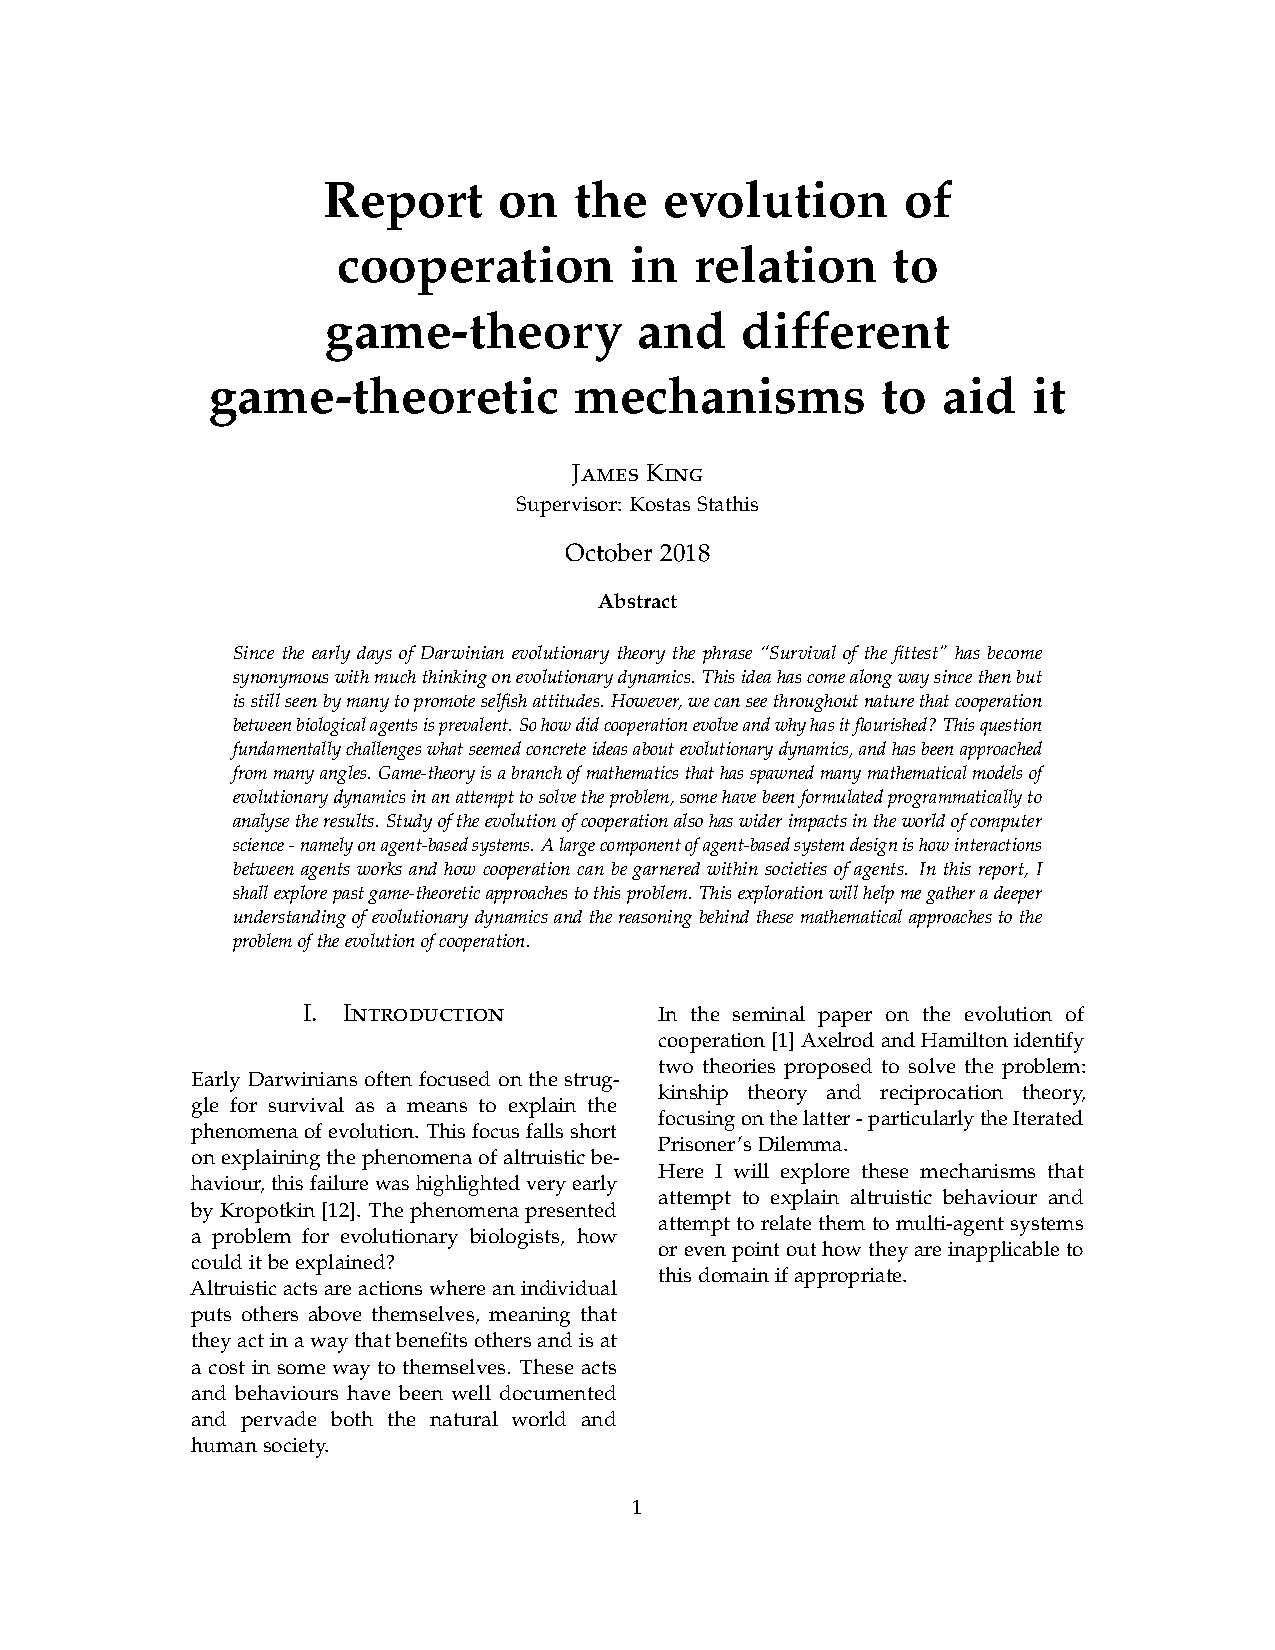
\includepdf[pages=-]{../../EvolCoop/EvolCoopReport.pdf}

%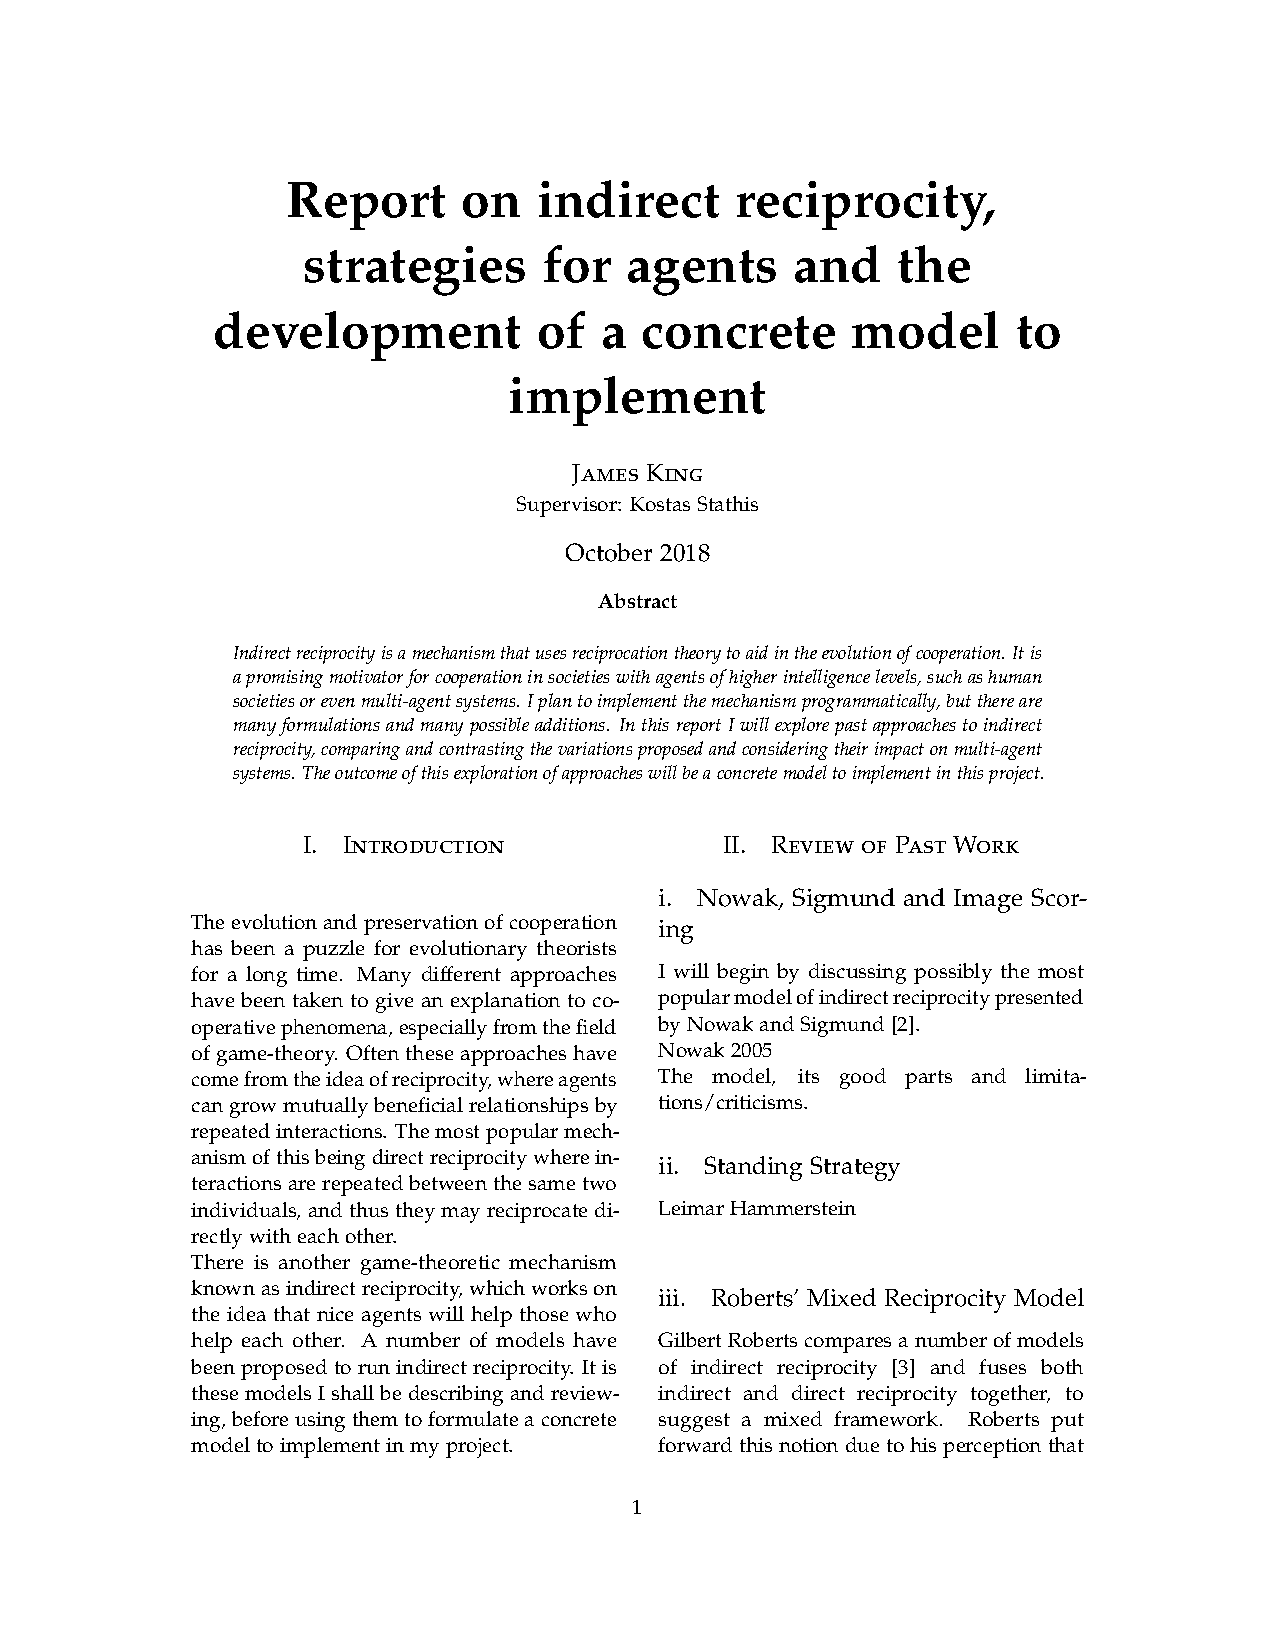
\includepdf[pages=-]{../../IndirRec/IndirRec.pdf}

%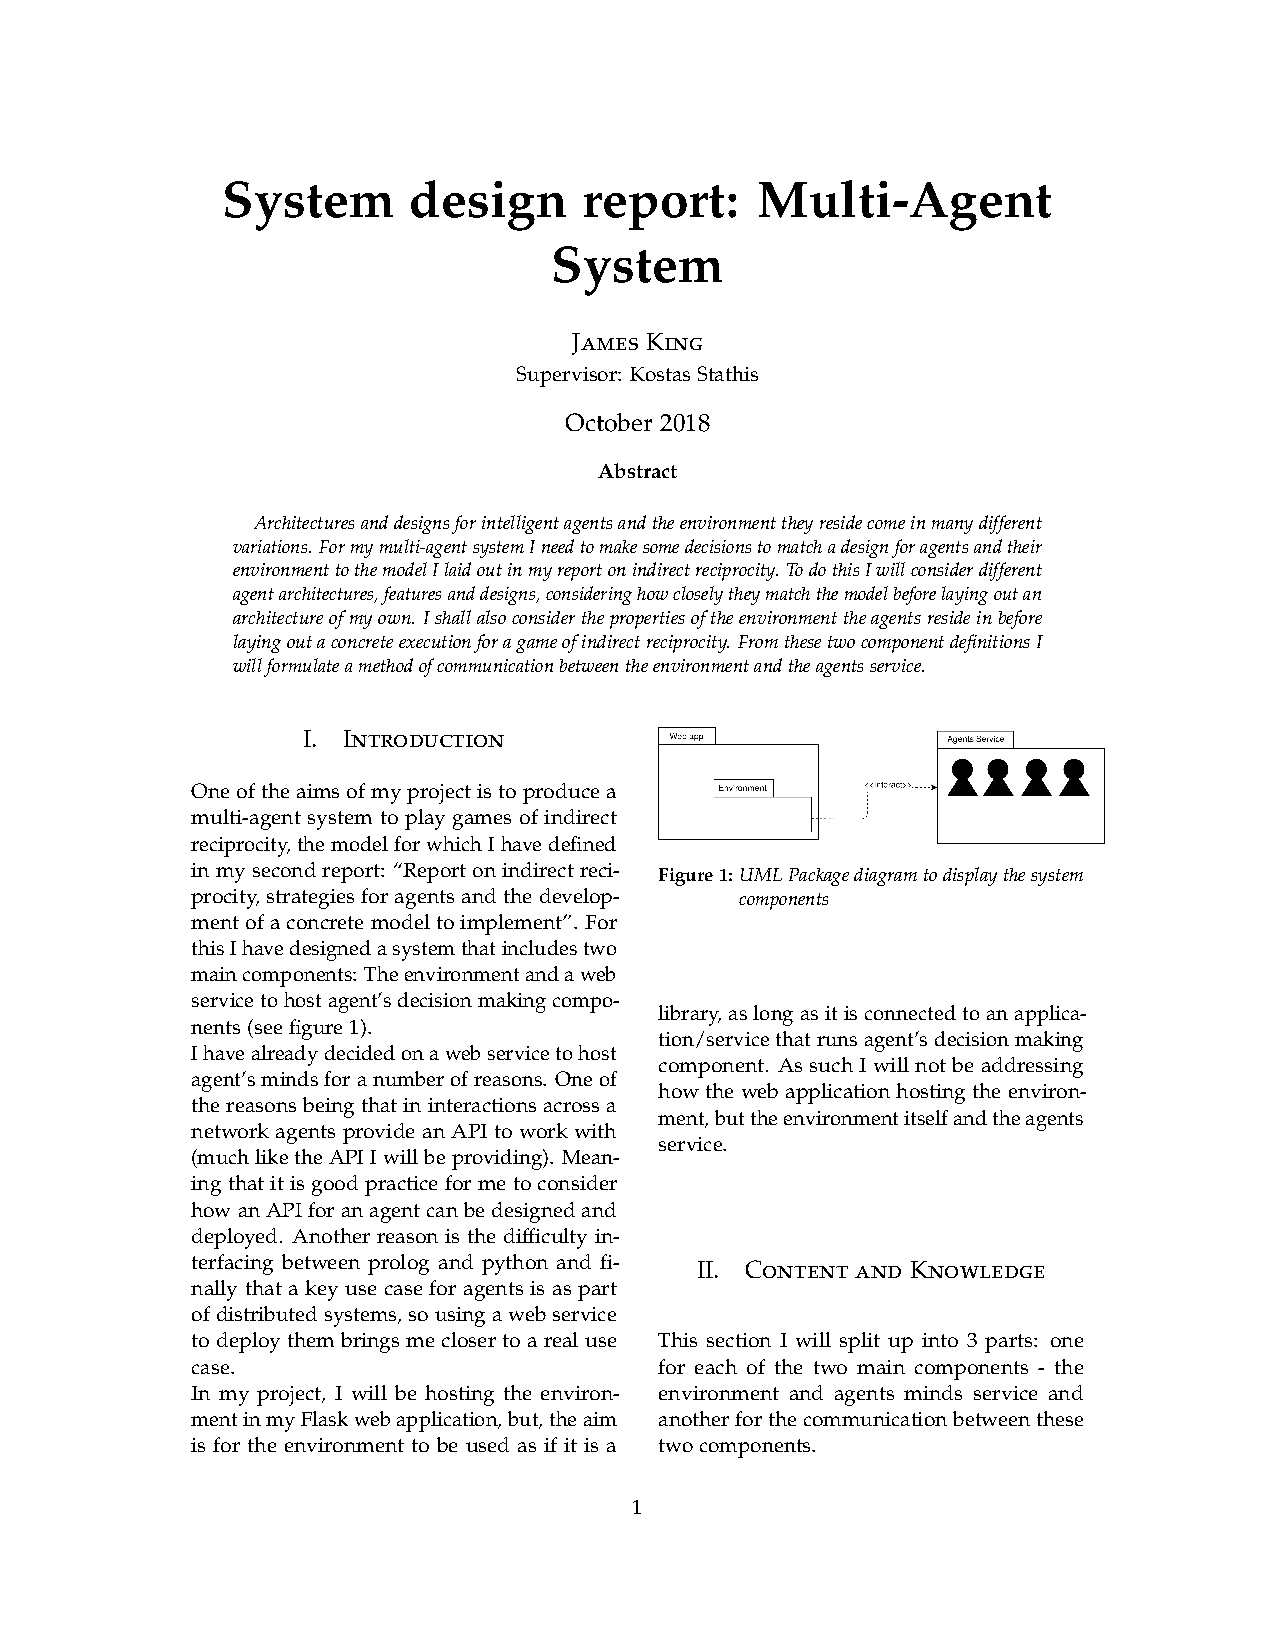
\includepdf[pages=-]{../../SysDesign/SysDesign.pdf}

\end{document}

\end{article}
